We present our work in two studies.  Study 1 provides a descriptive overview of the human predictions during the course of three rounds in the forecasting tournament, both in aggregate and idiographically (for some individuals).  This will provide a sense of the data structure and the performance of the forecasters.  The primary focus for Study 1, however, was to tackle our first objective: observe how participants adapt their predictions in real-time and to understand the relation between the unobservable theoretic component, the prior, and the human predictions.  Study 2 addressed our second objective: to explore possible relations between external data, the human predictions and, potentially, to components of the rational model (e.g., the prior).  To this end, we used the same human predictions from Study 1 and provided an analysis of the relation of the human predictions to the epidemiological case-count in Virginia. Next, we provide general methodological details that apply to both studies prior to detailing the specific methods used in each study.

\subsection{Forecasting Interface}\label{interface}
Participants were not restricted in terms of the number of forecasts they could make, given they were within the forecasting window (the window of time for which forecasters were permitted to submit predictions).  The interface presented to participants the prediction window of the question (the window of time for which predictions were made) as a timeline; overlaying the timeline was a visual representation of a probability density distribution (logistic in form).  The participant entered a forecast by manipulation of three horizontal sliders, two of which adjusted the width (left, right) of the probability distribution and one of which adjusted its center.  Further, the participants could generate a mixture distribution for their prediction as a layered and weighted combination of up to five separate distributions.  
%MUST GET ANSWER ON NON-SYMMETRY OF HAND GENERATED FUNTION VS LOGISTIC.
%Formally, this is:
%\begin{equation}
%    f(x) = \sum_{k=1}^{5} \pi_k g(x\vert \mu_k,s_k)
%\end{equation}
%where $\pi$ represents weights for each of the five (up to five) distributions.  Each distribution was defined as:
%\begin{equation}
%    g(x\vert \mu_k,s_k) = \frac {e^{-x(x-\mu)/s}} {s(1+e^{-x(x-\mu)/s})^2}
%\end{equation}
%The \pi_i were constrained so that their sum was $\le$ 1.
In addition to the visual of the prediction distribution, the participant saw the median, and quartiles of the distribution both visually (as vertical lines in the probability distribution) and numerically.  The questions under investigation in this article were discrete in nature (day); the numerical value of the prediction was presented at the day resolution to the participant as a summary measure of the participants probability distribution.  

\subsection{Data Structure and Major Constructs}\label{data-structure}
These data were extracted from the first three rounds of an online prediction tournament run by Metaculus and using the Metaculus forecasters pool as the participants (we describe the pool in section Participants).  The dates available for forecasting (the forecasting window) per rounds 1-3 were, respectively: 11-12-2021 to 12-03-2021; 12-03-2021 to 12-24-2021; 12-24-2021 to 01-14-2022.  The prediction window (the horizon of the forecast) for the forecasts per rounds 1-3 were, respectively: 11-12-2021 to 02-03-2022; 12-03-2021 to 02-25-2022; 12-24-2022 to 03-18-2022.  Each forecast made by a participant was in answer to the following question:  "When will the peak .. occur ". For the remained of this article, we call this the duration of the epidemic as short-hand for the duration from start to the peak of the epidemic curve. 

To generate $t_{past}$ we defined $t_0$ to be the beginning of the Omicron wave of COVID-19 and set it to November 29, 2021; this date was based on a reasonable estimate considering the daily reported case-count curve in Virginia (see \cite{VDHOnline}).  To construct $t_{predicted}$ for each forecast, we first transformed the participant input to the forecasting interface (described above) into a single date value that approximated the observed median of a prediction.  The data structure provided by the forecasting interface was in the form of a discrete probability mass function of ordered time intervals over an 84 day prediction window.  This generated 101 evenly spaced time intervals of the length of 20 hours, 9 minutes and 36 seconds (this interval times 101 = 84 days) each with a probability.  We defined the median of the prediction to be the discrete value $X$ for which $X \le 0.50$ when transforming the discrete probability mass function into a cumulative probability mass function.  In short, this procedure defined a single value, the approximate median value, as predicted date. Then, to construct $t_{predicted}$, we subtracted $t_0$ from the predicted date (e.g., Jan 2, 2022 minus November 29, 2021 $= t_{predicted}$ of 34 days).  Further, another useful construct is the prediction horizon, what we call the \textit{human horizon}; we defined this to be the number of days between the date on which a prediction was generated and the predicted date of the prediction.  This measure was useful because it represents the distance between $t_{past}$ and $t_{predicted}$ directly, a measure that theoretically important in terms of the potential for the rational prediction model to generates seemingly paradoxical behavior, as described in the Introduction.  In particular, in our analysis we were concerned with behavior of the rational model when the horizon was small.  We also extracted the date the prediction was generated by the participant, a measure that did not require transformation.

In short, the forecasting tournament data provided the date the prediction was generated by the participant (e.g., December 20, 2021) and the predicted date of the epidemic peak (e.g., Jan 2, 2022). Given a pre-defined beginning of the epidemic curve, $t_0$, we could generate both $t_{past}$ and $t_{predicted}$ as required by our theoretical model.  Further, we use the human horizon to understand the relation between the human predictions and the rational model when the human horizon is small.

The other major data structure reflected a measurement of the daily-case count for COVID-19 in Virginia.  These publicly available data were provided by the Virginia Electronic Disease Surveillance System (VEDSS) \citep{VDHOnline} and are entered by 5:00 PM the prior day (but are subject to change as quality assurance was ongoing).  VEDSS adopted the CDC COVID-19 2021 Surveillance Case Definition \citep{CDCguide} on September 1, 2021.  The quality assurance methods for VEDSS in respect to these data can be accessed here \citep{VDHquality}.

The raw form of these data is the cumulative number of cases on each day.  We transformed this into the daily number of cases per day by computing daily differences.  We then computed the rolling seven-day average over these raw data.  Because we had data for days well beyond both end-points of interest (11-30-2021 and 01-14-2022), our data structure on those days reflects the rolling seven day average prior to and after those end-points where appropriate.

\subsection{Participants}\label{participants}
All participants were users on the Metaculus forecasting platform (see \citep{metaculus}).  Metaculus is an online platform that hosts a community of forecasters (N is approximately 15,000). It is publicly accessible (with free registration for an active account) and hosts individual questions and tournaments with monetary prizes.  The Metaculus platform does not collect demographic data on the forecasters.  Further, for the participants reported in this article, we could not access summary information on the distribution of competence from prior forecasts. 

\subsection{Pre-processing of Forecasts}
The design of the forecasting tournament necessitated some pre-processing of these data; we selected/filtered based on criteria applied to the predictions not to participants. We started with 471 predictions that were generated by 47 participants.  The first step was to filter out predictions that were using the end-points of a round's prediction window, what we dub end-point forecasts; left end-point forecasts were at the earliest point of the prediction window; right end-point forecasts were at the latest point.  Because the prediction windows were bounded, we could not know if a end-point forecast was for the endpoint or beyond it.  None of the predictions fit this criteria.  The second step was to filter out the predictions that were prior to our definition of the start of the epidemic wave, $t_0$.  This reduced the number of predictions to 403 and the number of participants to 39.  The final filtering process was to remove predictions that were less than $t_{past}$ because these are theoretically impossible (impossible by the theory).  This removed two predictions for a final usable total of 401 predictions generated by 39 participants.  The distribution of the number of forecasts per user was highly right-skewed (mean=10.33, std=15.98, median=3, skew=2.15).

\subsection{Key Features of the Theoretical Model}
Our theoretical model, described in the Introduction, was borrowed directly from \citep{GriffithsTenenbaum2006} and differed only in its implementation (we describe the implementation in the next section).  We describe two key features of the model here: (i) the paradoxical \textit{prior crash} that was outlined briefly in the Introduction and (ii) the theoretical integration of new observations into the decision process and how statistically independent and dependent observations effect the model differently.  

\subsubsection{Invariant Predictions vs Invariant Priors}
We introduced the somewhat paradoxical feature of the Bayesian decision model when $t_{past}$ approaches $t_{predicted}$ in the Introduction.  Here we provide a detailed description of how this operates (please refer to Equation \ref{eq:posteriorfori} for this discussion).    This is best illustrated via an hypothetical example.  A person, Pat, is traveling on a train on a familiar route. After 20 minutes from departure, Pat is asked by another passenger how long will the train trip last (i.e., what will be the total duration in minutes).  For this example, $t_{past}$ is 20 minutes and $t_{total}$ is one value from a distribution encoded in memory by Pat's past experience on this train route, e.g., 45 minutes. Pat's response, according to the Bayesian decision model, is formulated as the expected value of the probability distribution generated from Equation \ref{eq:posteriorfori} over the distribution of all $t_{total}$. We call this decision $t_{predicted}$ to capture the notion that the rational model predicts a value of $t$ to be the duration of the current train trip.  In Bayesian terms, $P(t_{total})$, over all instances of $t_{total}$, defines the prior distribution; $P(t_{past} \vert t_{total})$ is the likelihood; $P(t_{total} \vert t_{past})$, over all instances in the prior, is the posterior distribution for a single value of $P(t_{past})$.

Let us continue on our journey with Pat.  Imagine that Pat is riding on a train and is probed to provide a prediction of the duration of the trip (i.e., $t_{predicted}$) at at a frequency of once per minute.  Further, assume that Pat generates an invariant value for $t_{predicted}$ of 50 minutes whenever probed.  In this scenario, a conclusion of the rational model is that Pat's prior must decrease as $t_{past}$ approaches $t_{predicted}$. This scenario is illustrated in the top panel of Figure \ref{fig:PriorShift2Panel}.  Put simply, by the rational prediction model, Pat's prior must decrease rapidly when Pat's prediction is invariant.  Figure \ref{fig:PriorShift1} shows the time evolution of the prior under this scenario, something that is recoverable if we know both $t_{past}$ and $t_{predicted}$. What we see here is that to maintain an invariant $t_{predicted}$ as $t_{past}$ approaches it, the prior distribution shifts rapidly to the left.   

Another side of this paradoxical feature of the rational model is the limiting case when the prior is fixed (shown in the lower panel of Figure \ref{fig:PriorShift2Panel}), the prediction $t_{predicted}$ increases as $t_{past}$ approaches it.  For this case, we imagine that Pat has an invariant prior the effect of which is that Pat's prediction of when the train trip will end, $t_{predicted}$, increases as $t_{past}$ approaches it.  This is similar to asking Pat a different but common question. Imagine we ask Pat to predict a person's life-span; as $t_{past}$ (the current age of a person) approaches the expected value of the prior, the predicted life span increases--e.g., given that someone is 79 years of age (the expected value in the US \cite{Arias2019}), Pat's prediction, given the rational decision model, is a bit greater than 79.

\begin{figure}
    \centering
    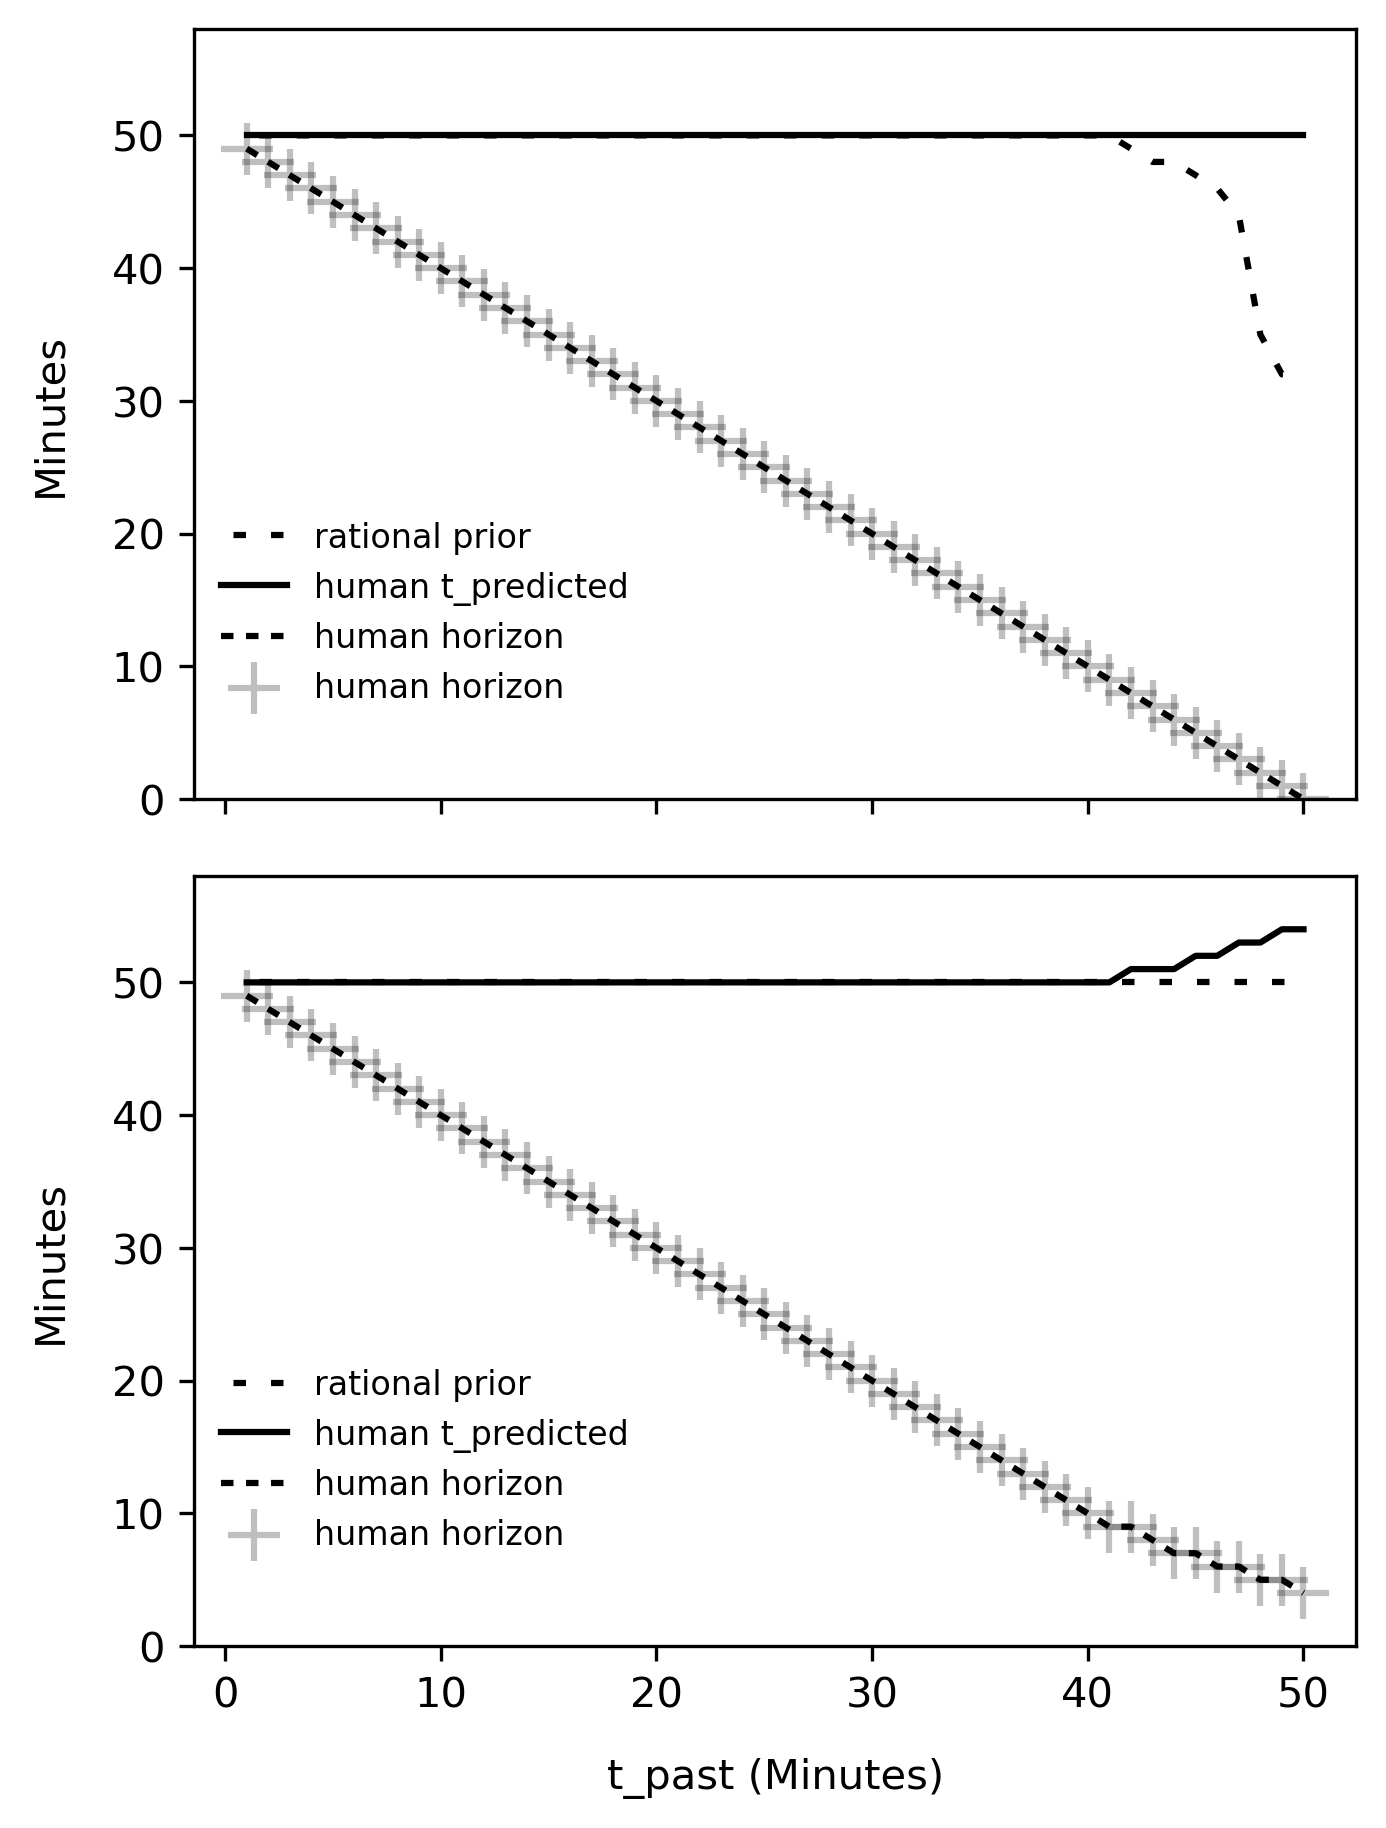
\includegraphics[width=0.75\textwidth]{Figures/Theory_PriorShift_1_2panel.png}
    \caption{\footnotesize{The theoretical relation between rational priors, $t_{past}$ and $t_{predicted}$ given the rational decision model for a hypothetical human riding on a train.  The x-axis represent the time at which a prediction is made, $t_{past}$;  the black, solid line represents the human decision, $t_{predicted}$; the black, large dashed line shows the prior, given $t_{past}$ and $t_{predicted}$, generated by the rational decision model; the human horizon reflects the amount of time until the predicted event from $t_{past}$ (i.e., its how far forward is the prediction from the moment it is given).  The top panel illustrates the invariant human decision case (a fixed $t_{predicted}$); as $t_{past}$ approaches $t_{predicted}$, the prior necessarily drops (what we call the "prior crash").  The lower panel shows the invariant prior case (a fixed prior distribution); as $t_{past}$ approaches $t_{predicted}$, $t_{predicted}$ increases.  
    }}
    \label{fig:PriorShift2Panel}
\end{figure}
%%%%
\begin{figure}
    \centering
    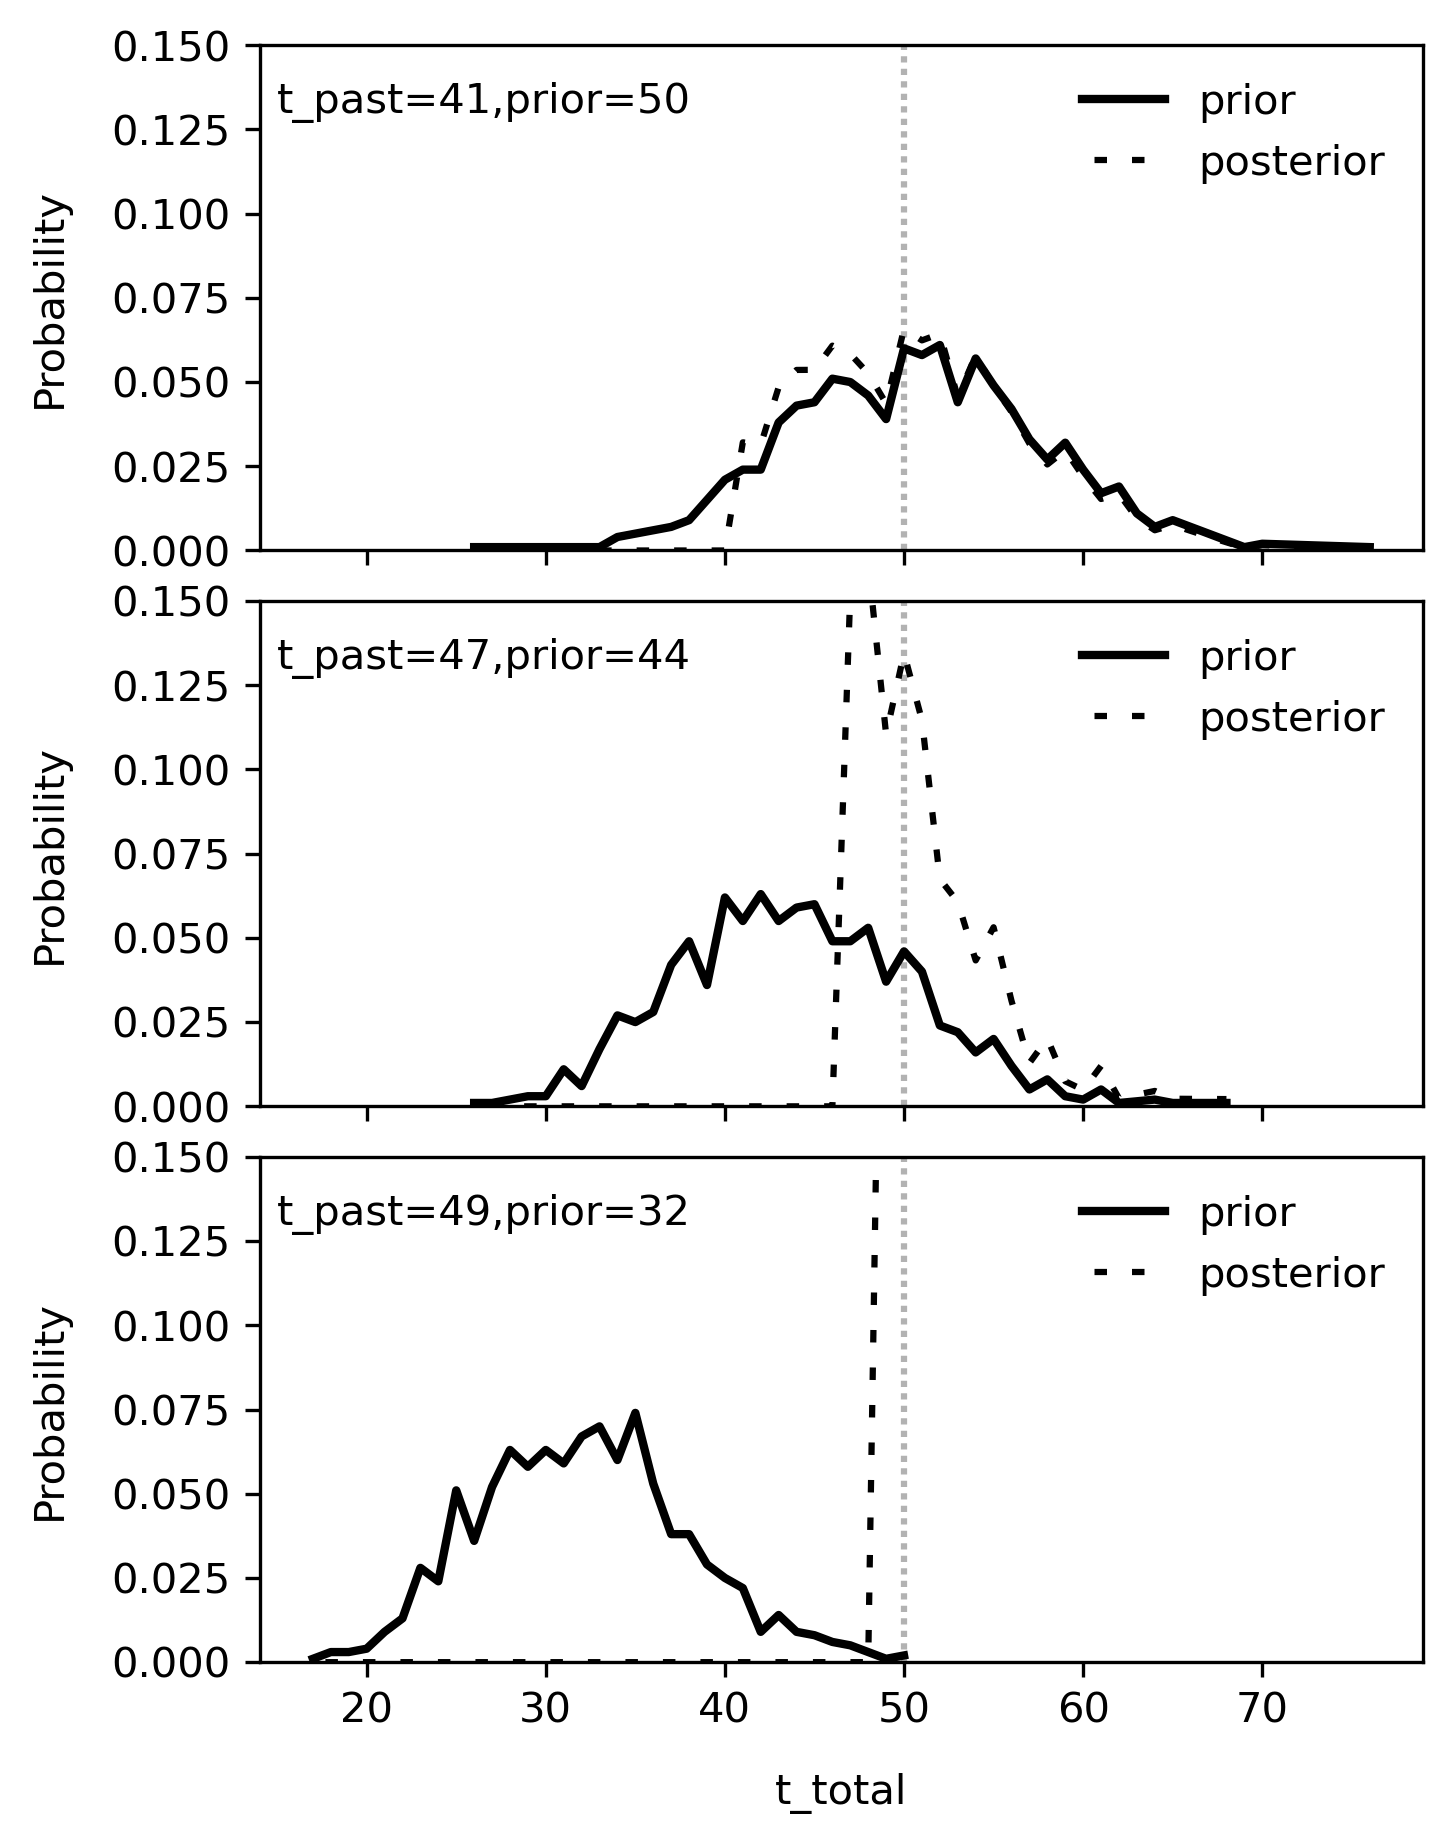
\includegraphics[width=0.75\textwidth]{Figures/Theory_PriorShift_1.png}
    \caption{The relation between prior and posterior distributions given three instances of the rational decision model; these instances were derived from the scenario shown in the top panel of Figure \ref{fig:PriorShift2Panel} for the condition of an invariant human decision, $t_{predicted}$, while riding on a train.  In each panel, the black solid line shows the posterior distribution; the black large dashed line shows the posterior distribution; the vertical grey small dashed line annotates the fixed invariant decision of 50 minutes.  Moving from the top to the bottom panel, this figure shows the leftward shift in the prior as $t_{past}$ increases from 41 to 47 to 49 minutes.  During this shift the median of the prior distribution shifts from 50 to 44 to 32 minutes while the median of the posterior distribution is maintained at 50 minutes.
    }
    \label{fig:PriorShift1}
\end{figure}

\subsubsection{The Integration of New Observations}
The integration of new observations, in terms of the decision model, operates on the likelihood function defined as:
\begin{equation}\label{eq:likelihoodN}
   \left(\frac{1}{t_{total}} \right)^n
\end{equation}
(when $t_{total} \ge t_{past}$) where $n$ is the number of observations (see \cite{GriffithsTenenbaum2011} p. 729 for derivation).  Thus, as the number of observations increases, the predicted $t_{predicted}$ decreases, assuming the prior is invariant.  This is the assumed case for statistically independent observations.  However, the experimental evidence suggested that for dependent observations, $n$ is effectively equal to one, suggesting provisionally that humans are sensitive to the generating process of new observations \citep{GriffithsTenenbaum2011}.  In short, the theoretical model and associated experimental results suggest that only independent observations can effect change in the likelihood. 

We raise this issue here because our observational context yielded repeated forecasts for individuals that are statistically dependent.  In reference to our hypothetical example, this is akin to asking Pat (from the example above) to predict the length of a single train trip repeatedly over the course of the trip at different values of $t_{past}$.  



\subsection{Methods: Study 1}
Our methodology was descriptive but in a manner that included the theoretical unobservable constructs of the Bayesian decision model.  We observed participants predictions from the forecasting tournament in real-time, both in aggregate and as individuals, and recovered the priors implied by the rational decision model.  This afforded a view of the dynamics of human predictions and their respective priors over the course of the tournament.  In particular, we observed conditions such that $t_{past}$ approached $t_{predicted}$ and thus served our first objective well.  We describe next the method for recovering the prior from the participant forecasts. 

\subsubsection{Recovering the Prior from Observations}
The primary use of the theoretical model in Study 1 was to recover the best prior given a participant's prediction, $t_{predicted}$, and the value of $t_{past}$ at the time of the participant's prediction.  Our theoretical model, described in the Introduction, was borrowed directly from \citep{GriffithsTenenbaum2006} and differed only in its implementation. We used a discrete, sampled prior and numerically computed the prior probability mass distribution from it; the likelihood was also computed from the same probability mass distribution.  Specifically, we used the Poisson distribution for the priors with the following probability mass function: 
\begin{equation}\label{eq:poisson}
   P(X=k) =  \frac {\lambda^k e^-{\lambda}}{k!.}
\end{equation}
where $k$ was the number of days and $\lambda$ was the expected number of days in an epidemic wave.  For each value of $\lambda$, across the range from 20 to 200 days, we generated 1000 samples numerically, using the scientific software 'Numpy'\footnote{We decided to use numerical samples in place of exact results to allow for a simple method for integrating sample biases into future modeling efforts or for integrating empirical estimates of real infectious disease wave durations.} from which we could compute the sampled probability mass function over the values of $k$ that were sampled numerically for a given $\lambda$.  This had the effect of restricting the prior and likelihood to the sampled values, but we desired a simple, approximate value for this study.

To find the prior distribution that was the best candidate for generating the human prediction $t_{predicted}$, we generated a three-way table that represented all combinations of prior distributions (medians of), $t_{past}$, and the median of the Bayesian decision model output $t_{predicted}$\footnote{Note that $t_{predicted}$ can refer to the human decision or the output of Bayesian decision model; this term will be used for both interchangeably} for the values constrained by the expected values $\lambda$ of our priors (20 to 200 days).  To recover the best candidate prior for a human prediction, we searched the three-way table for the closest match--i.e., we found the prior distribution that would have generated $t_{predicted}$ given $t_{past}$.  For purposes of analysis, we reported the expected value of the prior's distribution as the measure for analysis. Henceforth, we call this measure the prior; the context of our use of the term prior should help the reader to disambiguate the meaning of the expected value of the distribution from the distribution itself.  

By design, this method does not restrict a single prior to an individual over the course of the tournament, but only to a single prediction within the tournament; we wanted to see the extent to which an individual's prior varied over the course of the tournament, if at all.  

\subsection{Methods: Study 2}
Further, to serve our second objective, we provide an analysis of the relation between the human predictions and the Virginia daily-case count data of the COVID-19 Omicron wave.  This analysis relied on the rational decision model in the sense that it was the theoretical model that suggested to us a useful measure to extract from the tournament data: prediction in the form of $t_{predicted}$.  

This study used two data structures: (i) all 401 human predictions in terms of the predicted duration of the epidemic, $t_{predicted}$; (ii) the daily-case count for COVID-19 in Virginia, henceforth called case-count data.  

The human predictions were averaged by day (all predictions in a 24 hour period were averaged together) and then fitted using linear polynomial regression (where datetime was transformed to a linear variable as the predictor; we do not provide the coefficients here, but will report them upon request or they can be recovered by using our publicly available source code: \cite{orrgit}).  The purpose was to provide a relatively low-dimensional and smooth representation of the temporal signature of these data for our next processing step. Using the polynomial solution, we then computed, numerically, its first and second differentials.  We used the same method for the case-count data. 

In addition, we used a change-point method for the case-count data, based on the sequential discounting auto-regression learning (SDAR) algorithm \citep{Yamanishi2002}, to detect change points in the case-count data as we transformed it, prior to the polynomial fit, using a discount rate of 0.01, order of 3 and a smoothing factor of 5 days. 